\section{Experimental Results and Conclusions}

\subsection{Rule Learner}
We used 2000 randomly initialized board states each for our training, validation and testing datasets. All of these were valid board states and there were no repetitions.

We were able to achieve 100\% accuracy (0 Error) on the test set, where the error is the Euclidean distance between the predicted valid moves and actual valid moves (represented as cells containing either a 0 or a 1) averaged over all test set samples.

\subsection{Strategy Learner}
We trained this network over 150 epochs with 25000 episodes per epoch. This resulted in about 90000 games to train on. We were able to see the strategy network understand the valid moves input from the rule learner. To test the network we played against a random AI and a minimax algorithm with varying depths. The results can be seen in Table \ref{table}. 

\begin{table}[h!]
  \begin{center}
    \begin{tabular}{c||c}
    	opponent & result\\
    	\hline
    	\hline
      	random & 95$\%$\\
      	\hline
      	minimax 1 & win\\
      	\hline 
      	minimax 3 & win\\
      	\hline 
      	minimax 5 & lose\\
    \end{tabular}
  \end{center}
  \caption{Performance of the Strategy Learner against different opponents.}
  \label{table}
\end{table}

For the random result we would expect that there are situations that would arise that the network was not trained for and would lose. For the other results, against the minimax algorithm, only one game was played because both our network and the minimax algorithm are deterministic. 

A minimax at a depth of 10 is considered optimal, as it balances searching the tree and speed of the algorithm, however we found that the network was not able to learn a strategy that could beat the minimax at a depth of 5 let alone 10.

The strategy that the network learned does not always pick the optimal move. For example, in the situations below, it should have picked the winning move, but the network does not seem to learn how to win in all situations. This is demonstrated in Figures \ref{state_move_0} and  \ref{state_move_2}.

\begin{figure}
    \makebox[\linewidth]{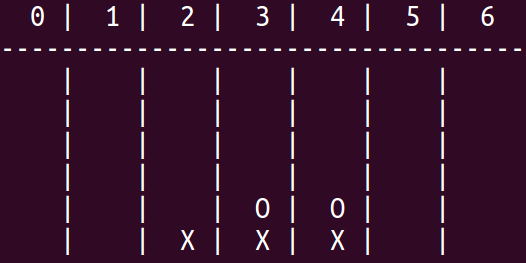
\includegraphics[width=0.5\textwidth]{state1.png}}
    \caption{A state in a game between minimax 3 and our trained network}
    \label{state_move_0}
\end{figure}


\begin{figure}
    \makebox[\linewidth]{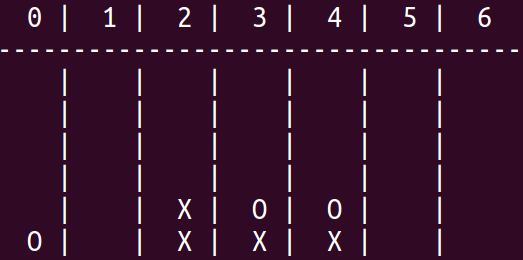
\includegraphics[width=0.5\textwidth]{state2.png}}
    \caption{A second state 2 moves later in a game between minimax 3 and our trained network}
    \label{state_move_2}
\end{figure}


Looking at these states we can see that the network could have won, however it did not pick the best result, confirming that currently the network is not optimal. However, we were able to improve upon random suggest future improvements could yield better results. 